\chapter{Protocol Analyzer View}

Some filters for decoding packet-oriented data provide an alternate means of visualizing the decoded traffic.

The protocol analyzer view (Fig. \ref{proto-analyzer}) displays each packet in the history as a row in a list view. The
first column is always the timestamp of the packet; remaining columns vary depending on the particular filter in
question.

Clicking on a packet pauses acquisition, loads the relevant waveform from history if the packet is not in the current
waveform, and scrolls the waveform view containing the protocol decode to the start of the packet. This allows
packet-level data to be easily correlated to physical layer waveforms.

If a vertical cursor is active in the waveform area displaying the protocol decode, clicking on a packet in the
analyzer view moves the cursor to the start of the packet. Placing the cursor on a packet highlights the corresponding
row in the protocol analyzer.

\begin{figure}[H]
\centering
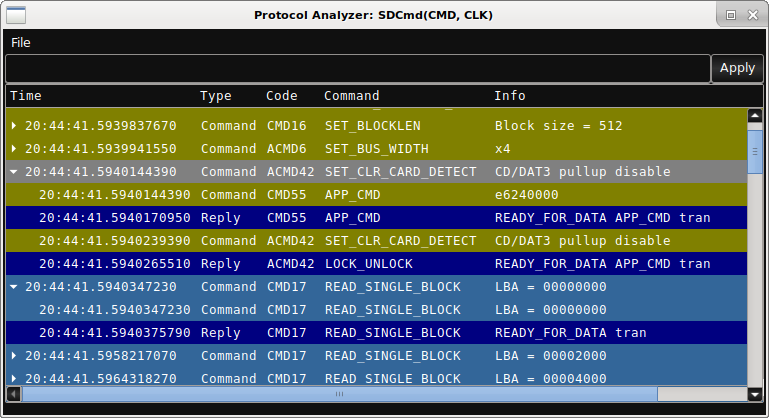
\includegraphics[width=14cm]{images/proto-analyzer.png}
\caption{Protocol analyzer view}
\label{proto-analyzer}
\end{figure}

Once closed, the protocol analyzer view may be reopened by selecting the protocol of interest from the
\menustyle{Window / Analyzer} menu.

Protocol packets are color coded according to the high-level function of the packet.

\begin{tabularx}{16cm}{llX}
\thickhline
\textbf{Color name} & \textbf{Use case} & \textbf{Default Color} \\
\thickhline
Command & Executing commands & \cellcolor{protocmd}\textcolor{white}{\#600050} \\
\thickhline
Control & Changing configuration & \cellcolor{protoctl}\textcolor{white}{\#808000} \\
\thickhline
Data read & Reading data & \cellcolor{protoread}\textcolor{white}{\#336699} \\
\thickhline
Data write & Writing data & \cellcolor{protowrite}\textcolor{white}{\#339966} \\
\thickhline
Error & Malformed, bad checksum & \cellcolor{protoerror}\textcolor{white}{\#ff0000} \\
\thickhline
Status & Status updates, flow control & \cellcolor{protostatus}\textcolor{white}{\#000080} \\
\thickhline
\end{tabularx}

Many filters group related packets (request and reply, escape sequences, polling loops, etc) under a single heading to
enable easier navigation of large datasets. The tree expansion button at the left of the timestamp column may be used to expand
the event into its constituent packets.
